\chapter{Block Propagation Delay Distribution}
\label{apx:propagation}

 Here we present the distribution plots of the block propagation delay ($\Delta$) in topologies tested in our scalability experiment (\S\ref{sec:eval-scale}). The data are shown in Figures~\ref{fig:propagation1}, \ref{fig:propagation2}, \ref{fig:propagation3}, \ref{fig:propagation4}, \ref{fig:propagation5}. In each plot, the concrete lines mark the mean of the propagation delay of that type of blocks, and the dashed lines mark the $25\%$ and $75\%$ quantiles. Comparing Figures~\ref{fig:propagation1}, \ref{fig:propagation3}, \ref{fig:propagation5} we observe that as long as the network diameter is kept constant, the block propagation delay is barely affected by the increase of clients.


\begin{figure}[t]
    \centering
    \begin{subfigure}{.5\textwidth}
        \centering
   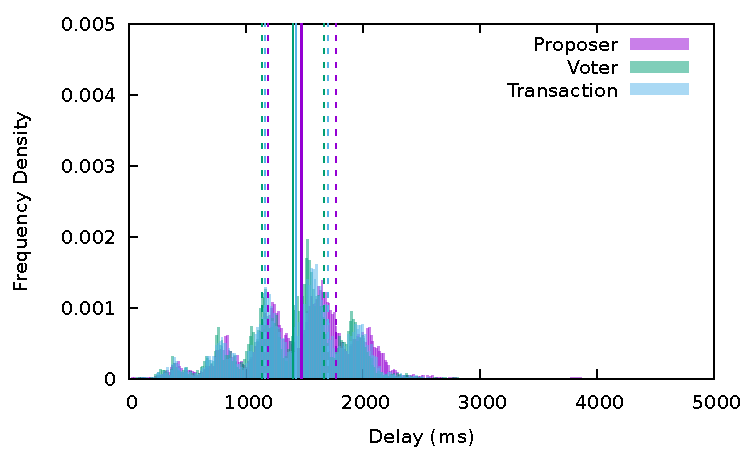
\includegraphics[width=\linewidth]{figures/delay100nodes.pdf}
   \caption{Nodes$=100$, Degree$=4$, Diameter$=5$}%\vspace{-6mm}
   \label{fig:propagation1}
    \end{subfigure}%
    \begin{subfigure}{.5\textwidth}
   \centering
   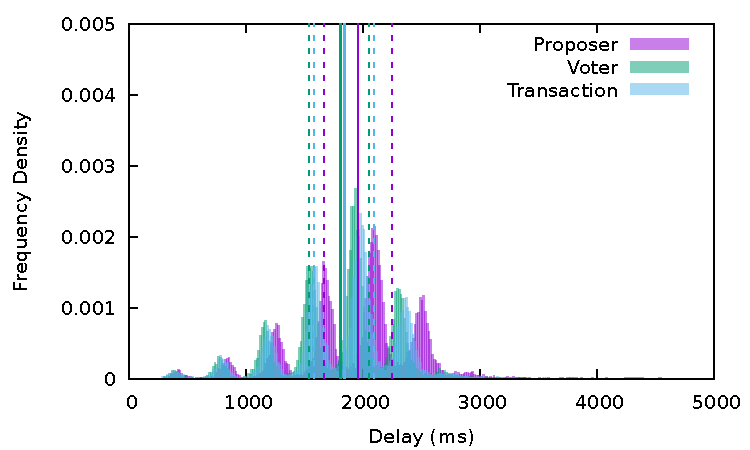
\includegraphics[width=\linewidth]{figures/delay300nodes4.pdf}
   \caption{Nodes$=300$, Degree$=4$, Diameter$=7$}%\vspace{-6mm}
   \label{fig:propagation2}
 \end{subfigure}%
    \newline
    \begin{subfigure}{.5\textwidth}
   \centering
   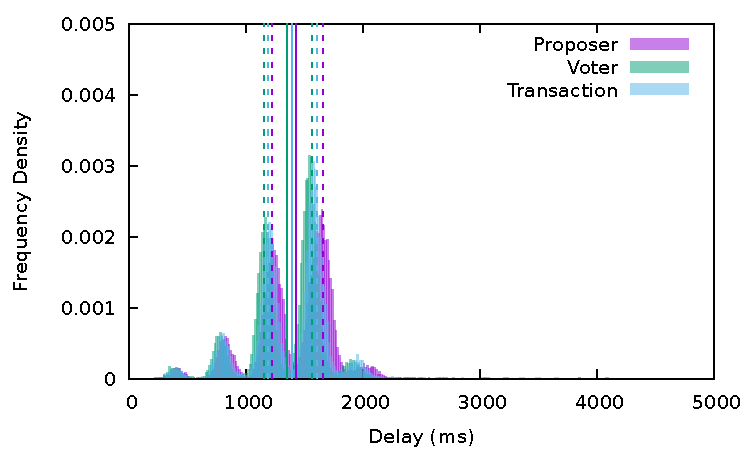
\includegraphics[width=\linewidth]{figures/delay300nodes6.pdf}
   \caption{Nodes$=300$, Degree$=6$, Diameter$=5$}%\vspace{-6mm}
   \label{fig:propagation3}
 \end{subfigure}%
    \begin{subfigure}{.5\textwidth}
   \centering
   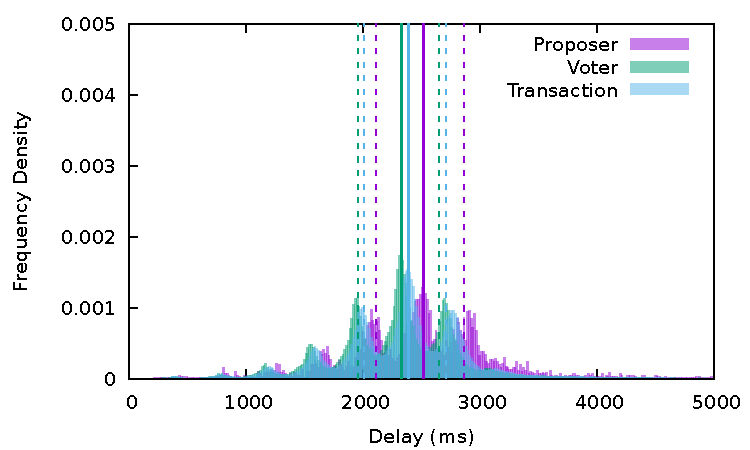
\includegraphics[width=\linewidth]{figures/delay1000nodes4.pdf}
   \caption{Nodes$=1000$, Degree$=4$, Diameter$=9$}%\vspace{-6mm}
   \label{fig:propagation4}
 \end{subfigure}%
    \newline
    \begin{subfigure}{.5\textwidth}
   \centering
   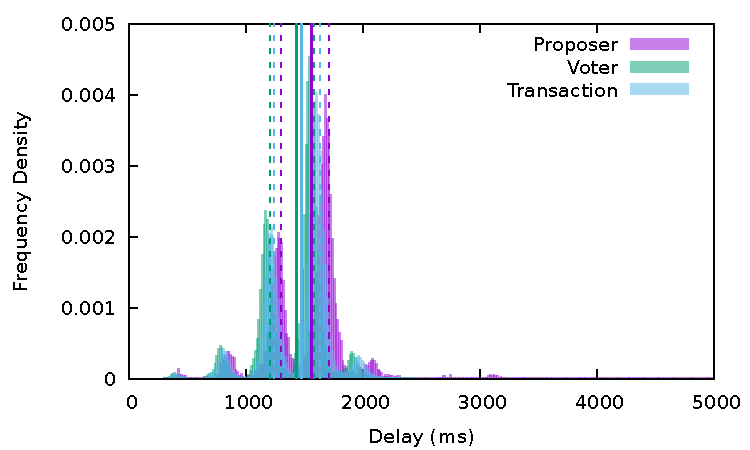
\includegraphics[width=\linewidth]{figures/delay1000nodes8.pdf}
   \caption{Nodes$=1000$, Degree$=8$, Diameter$=5$}
   \label{fig:propagation5}
 \end{subfigure}
 
    \caption{Block propagation delay in the testbed.}
    \label{fig:propagation}
\end{figure}
